\documentclass{zjureport}
% =============================================
% Part 1 Edit the info
% =============================================

\newcommand{\major}{测控技术及仪器}
\newcommand{\name}{郑成琦}
\newcommand{\stuid}{3179801017}
\newcommand{\newdate}{2020-4-8}
\newcommand{\loc}{家}

\newcommand{\course}{EDA技术应用}
\newcommand{\tutor}{黄添添}
\newcommand{\grades}{None}
\newcommand{\newtitle}{四位计数器设计}
\newcommand{\exptype}{设计与编码实验}
\newcommand{\group}{None}

% =============================================
% Part 1 Main document
% =============================================
\begin{document}
\thispagestyle{empty}
\begin{figure}[h]
  \begin{minipage}{0.6\linewidth}
    \centerline{\includegraphics[width=\linewidth]{head.jpg}}
  \end{minipage}
  \hfill
  \begin{minipage}{.4\linewidth}
    \raggedleft
    \begin{tabular*}{.8\linewidth}{ll}
      专业: & \underline\major   \\
      姓名: & \underline\name    \\
      学号: & \underline\stuid   \\
      日期: & \underline\newdate \\
      地点: & \underline\loc
    \end{tabular*}
  \end{minipage}
\end{figure}

\begin{table}[!htbp]
  \centering
  \begin{tabular*}{\linewidth}{llllll}
    课程名称: & \underline\course   & 指导老师: & \underline\tutor   & 成绩:       &  \underline\grades \\
    实验名称: & \underline\newtitle & 实验类型: & \underline\exptype & 同组学生姓名:& \underline\group
  \end{tabular*}
\end{table}

% =============================================
% Part 2 Main document
% =============================================

\section{实验目的和要求}
1、了解Quartus II开发环境,熟悉Verilog语言基本语法

2、实现4位计数器选择功能
\section{实验内容和步骤}

  \subsection{实验内容}
	根据所给的手册《My First FPGA》进行实验操作。最后在上述基础上加入计数选择功能。
  \subsection{实验步骤}
	\begin{clause}
		\item 加法器的HDL语言编写
		\item PLL模块调用
		\item Multiplexer模块调用
		\item 进行仿真
	\end{clause}
\section{主要仪器设备}
  计算机,Quartus

\section{操作方法和实验步骤}
  \subsection{加法器HDL语言编写}
    \lstinputlisting[language=Verilog]{FPGA_EDA_one/simple_counter.v}
  \subsection{PLL模块调用}
    (因为软件原因,模块显示在我的电脑是挤在一起十分混乱)
    \begin{clause}
      \item 模块图片
      \begin{center}
        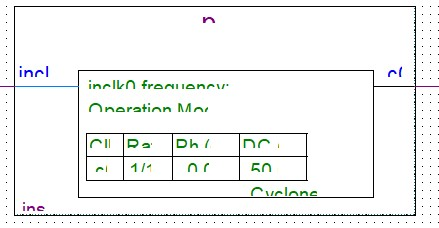
\includegraphics[width=0.6\linewidth]{PLL.jpg}
      \end{center}
      \item 模块连线 
      \begin{center}
        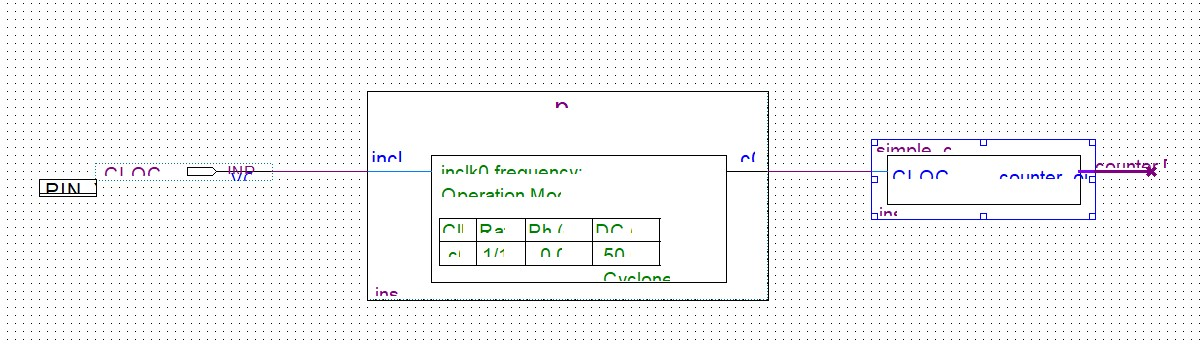
\includegraphics[width=0.6\linewidth]{figures/Link_1.jpg}
        \\PLL的输出作为计数器的输入来作为主要的计数速度控制手段。
      \end{center}
    \end{clause}
  \subsection{Multiplexer模块调用}
    
\section{实验数据记录和处理}
  \subsection{传输函数}
    根据差分方程,传输函数如下:
    $$H(z) = \frac{Y(z)}{X(z)} = \frac{z^2}{z^2-(0.5+a)z+0.5a}$$
  \subsection{零极点分布图}
    a = 0.8,0.9,1.1时,系统的零极点分布图及程序如下:
    \begin{clause}
      \item 图像
      \begin{center}
        \includegraphics[width=0.6\linewidth]{01.jpg}
      \end{center}
      \item 代码
      \lstinputlisting[language=MATLAB]{code/do.m}
    \end{clause}

  \subsection{频率响应}
    a = 0.8,0.9,1.0,1.1时,系统的频率响应函数图形及程序如下:
    \begin{clause}
      \item 图像
      \begin{center}
        \includegraphics[width=0.6\linewidth]{02-1.jpg}
      \end{center}
      \item 代码
      \lstinputlisting[language=MATLAB]{code/next.m}
    \end{clause}

\section{实验结果与分析}

balabalabala

\end{document}
